% Section
\section{Evaluation}
\label{sec:experiments}

The experiments presented hereafter evaluate the performance of our balancing methods when compared to an existing and effective task clustering strategy named Horizontal Clustering (HC)~\cite{Singh:2008:WTC:1341811.1341822}, which is widely used by workflow management systems such as Pegasus. We also compare our methods with two legacy heuristics from the literature: DFJS~\cite{Muthuvelu:2005:DJG:1082290.1082297}, and AFJS~\cite{Liu2009}. DFJS groups bag of tasks based on the �task durations up to the resource capacity. AFJS is an extended version of DFJS that is an adaptive fine-grained job scheduling algorithm to group fine-grained tasks according to processing capacity and bandwidth of the current available resources.

% Workflow applications
\subsection{Scientific workflow applications}
\label{sec:applications}

Five real scientific workflow applications are used in the experiments: LIGO~\cite{LIGO} Inspiral analysis, Montage~\cite{Berriman2004}, CyberShake~\cite{Graves2010}, Epigenomics~\cite{Epigenome}, and SIPHT~\cite{SIPHT}. 

\paragraph{\textbf{LIGO}}
The Laser Interferometer Gravitational Wave Observatory (LIGO) workflows are used to search for gravitational wave signatures in data collected by large-scale interferometers. The observatories' mission is to detect and measure gravitational waves predicted by general relativity ��Einstein's theory of gravity �in which gravity is described as due to the curvature of the fabric of time and space. LIGO Inspiral workflow is a data intensive workflow. Figure~\ref{fig:evaluation_shape_ligo} shows a simplified version of the workflow.

\begin{figure}[!htb]
	\centering
	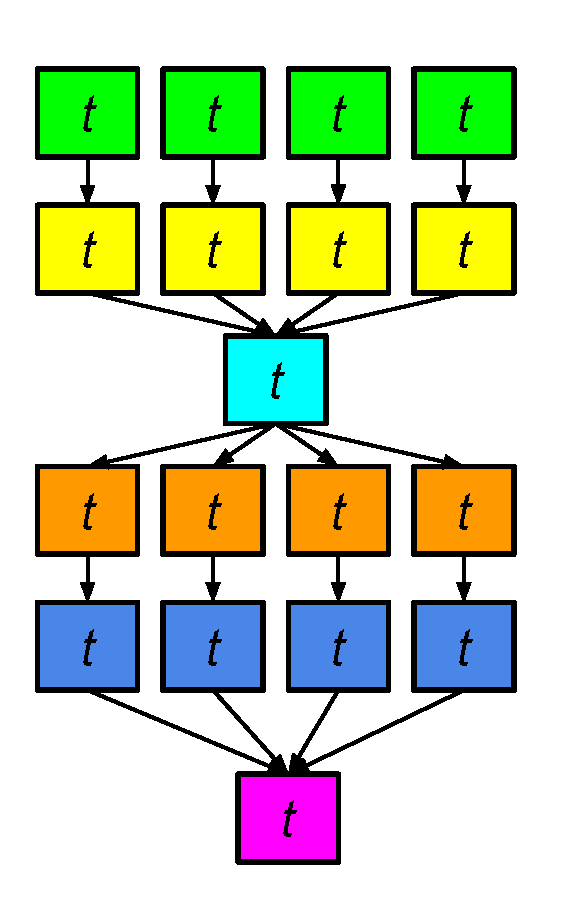
\includegraphics[width=0.6\linewidth]{figures/evaluation/inspiral.pdf} \\
	\caption{A simplified visualization of the LIGO Inspiral workflow.}
	\label{fig:evaluation_shape_ligo}
\end{figure}

\paragraph{\textbf{Montage}}
Montage is an astronomy application that is used to construct large image mosaics of the sky. Input images are reprojected onto a sphere and overlap is calculated for each input image. The application re-projects input images to the correct orientation while keeping background emission level constant in all images. The images are added by rectifying them into a common flux scale and background level. Finally the reprojected images are co- added into a final mosaic. The resulting mosaic image can provide a much deeper and detailed understanding of the portion of the sky in question. Figure~\ref{fig:evaluation_shape_montage} illustrates a small Montage workflow. The size of the workflow depends on the number of images used in constructing the desired mosaic of the sky. The structure of the workflow changes to accommodate increases in the number of inputs, which corresponds to an increase in the number of computational tasks.



\begin{figure}[htb]
	\centering
	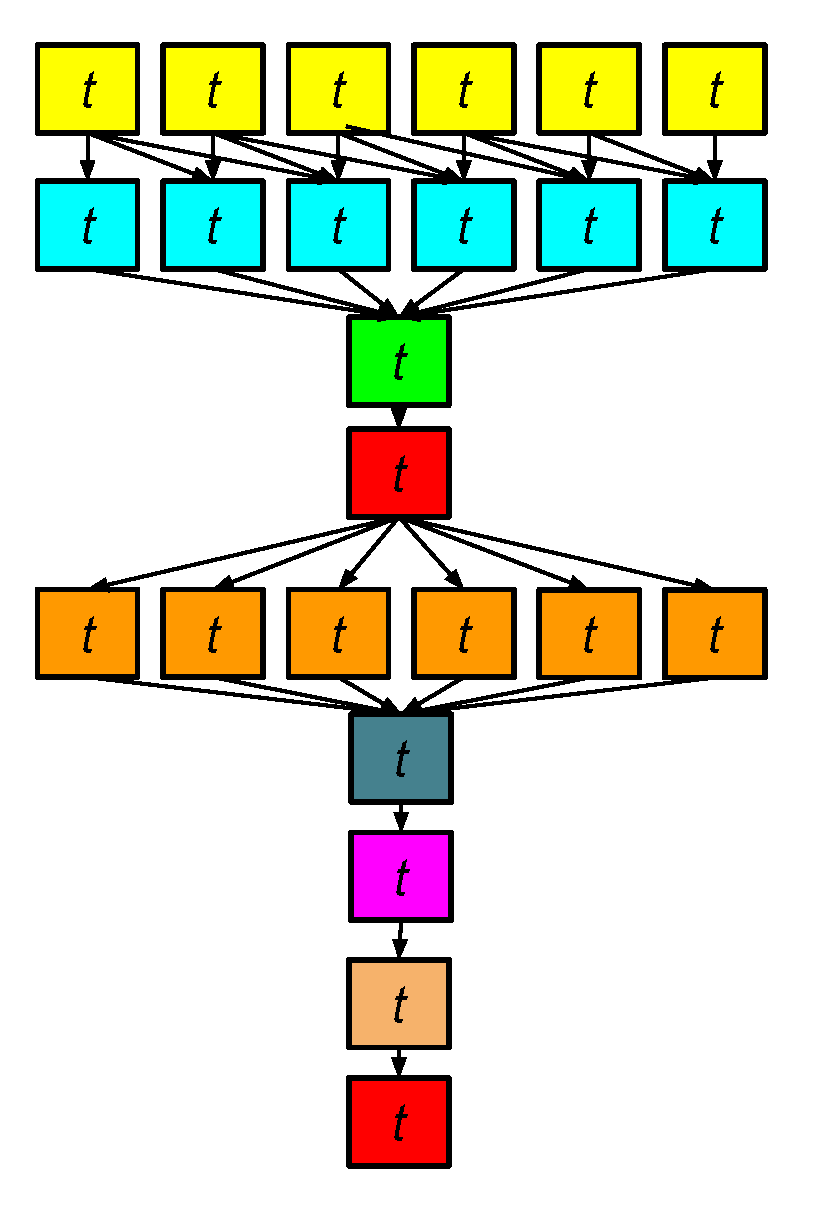
\includegraphics[width=0.55\linewidth]{figures/evaluation/montage.pdf} \\
	\caption{A simplified visualization of the Montage workflow.}
	\label{fig:evaluation_shape_montage}
\end{figure}

\paragraph{\textbf{Cybershake}}
CyberShake is a seismology application that calculates Probabilistic Seismic Hazard curves for geographic sites in the Southern California region. It identifies all ruptures within 200km of the site of interest and convert rupture definition into multiple rupture variations with differing hypocenter locations and slip distributions. It then calculates synthetic seismograms for each rupture variance and peak intensity measures are then extracted from these synthetics and combined with the original rupture probabilities to produce probabilistic seismic hazard curves for the site. Figure~\ref{fig:evaluation_shape_cybershake} shows an illustration of the Cybershake workflow.

\begin{figure}[htb]
	\centering
	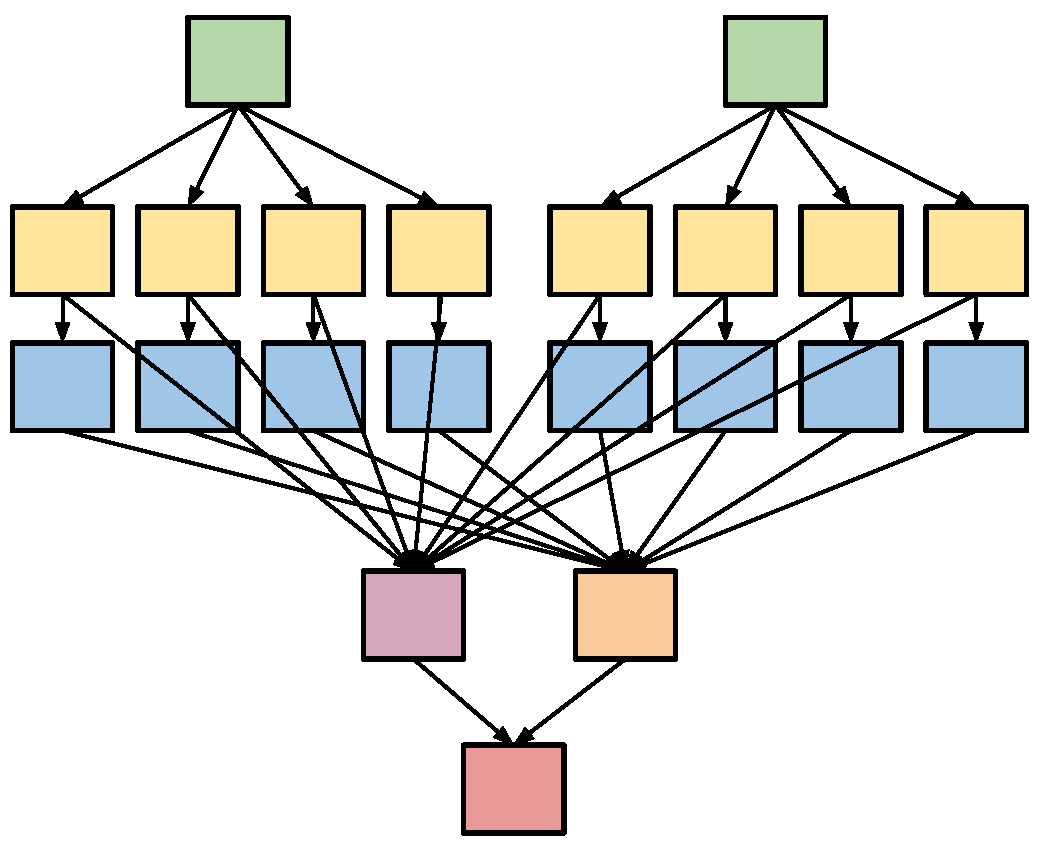
\includegraphics[width=0.7\linewidth]{figures/evaluation/cybershake.pdf} \\
	\caption{A simplified visualization of the CyberShake workflow.}
	\label{fig:evaluation_shape_cybershake}
\end{figure}

\paragraph{\textbf{Epigenomics}}
The Epigenomics workflow is a pipeline workflow. Initial data are acquired from the Illumina-Solexa Genetic Analyzer in the form of DNA sequence lanes. Each Solexa machine can generate multiple lanes of DNA sequences. These data are converted into a format that can be used by sequence mapping software. The mapping software can do one of two major tasks. It either maps short DNA reads from the sequence data onto a reference genome, or it takes all the short reads, treats them as small pieces in a puzzle and then tries to assemble an entire genome. In our experiments, the workflow maps DNA sequences to the correct locations in a reference Genome. This generates a map that displays the sequence density showing how many times a certain sequence expresses itself on a particular location on the reference genome. Scientists draw conclusions from the density of the acquired sequences on the reference genome. Epigenome is a CPU-intensive application and its simplified structure is shown on Figure~\ref{fig:evaluation_shape_genome}. 

\begin{figure}[htb]
	\centering
	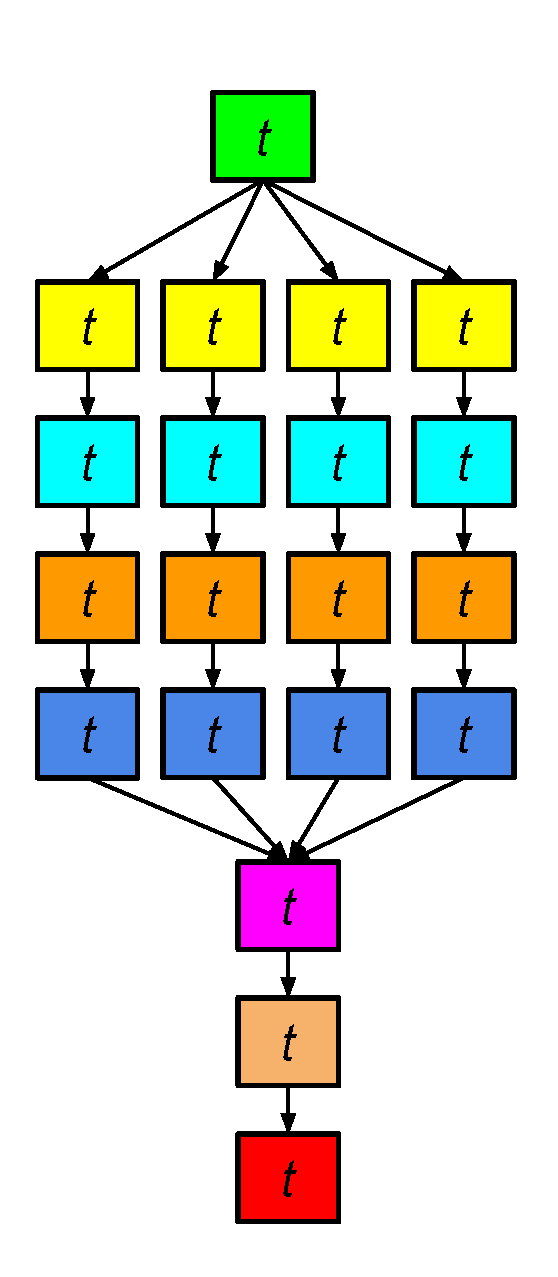
\includegraphics[width=\linewidth]{figures/evaluation/genome.pdf} \\
	\caption{A simplified visualization of the Epigenomics workflow.}
	\label{fig:evaluation_shape_genome}
\end{figure}

\paragraph{\textbf{SIPHT}}
The SIPHT workflow is conducting a wide search for small untranslated RNAs (sRNAs) that regulate several processes such as secretion or virulence in bacteria. The kingdom-wide prediction and annotation of sRNA encoding genes involves a variety of individual programs that are executed in the proper order using PEGASUS. These involve the prediction of Rho-independent transcriptional terminators, BLAST (Basic Local Alignment Search Tools) comparisons of the inter genetic regions of different replicons and the annotations of any sRNAs that are found. A simplified structure of the SIPHT workflow is shown on Figure~\ref{fig:evaluation_shape_sipht}. 

\begin{figure}[htb]
	\centering
	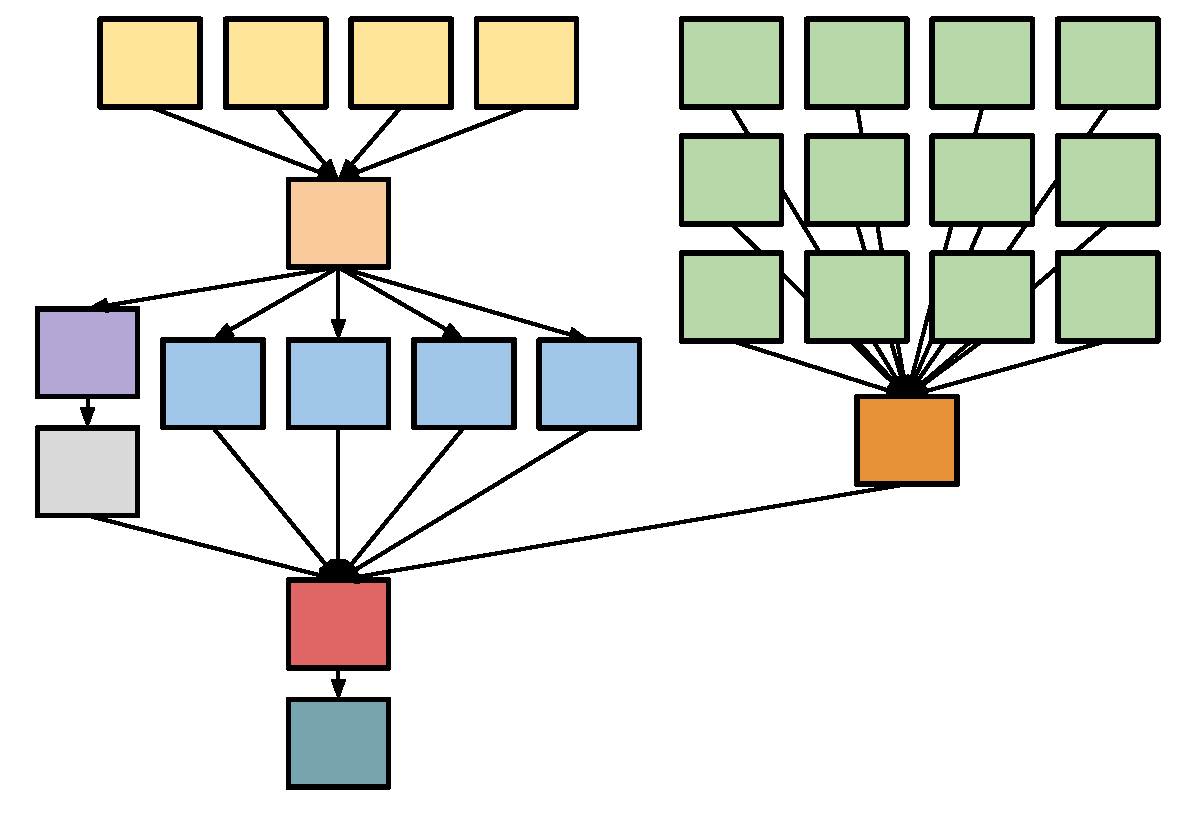
\includegraphics[width=0.7\linewidth]{figures/evaluation/sipht.pdf} \\
	\caption{A simplified visualization of the SIPHT workflow.}
	\label{fig:evaluation_shape_sipht}
\end{figure}

Table~\ref{tab:evaluation_workflows} shows the summary of the main workflows characteristics: number of tasks, average data size, and average task runtimes. 

\begin{table*}[!htb]
	\centering
	\small
	\begin{tabular}{lrrrr}
		\hline
		Workflow & Num of Tasks & Average Data Size &  Average Task Runtime \\
		\hline
		LIGO 		&800		& 5 MB	&228s\\
		Montage 		&300		&3 MB	&11s\\
		CyberShake 	&700		&148 MB 	& 23s\\
		Epigenomics 	&165 		& 355 MB	&2952s\\
		SIPHT		&1000		& 360KB & 180s\\
		\hline
	\end{tabular}
	\caption{Summary of the scientific workflows characteristics.}
	\label{tab:evaluation_workflows}
\end{table*} 



% Task clustering techniques
\subsection{Task clustering techniques}

In the experiments, we compare the performance of our methods to the Horizontal Clustering (HC)~\cite{Singh:2008:WTC:1341811.1341822} technique, which is widely used by Pegasus, and with two methods from the literature, DFJS~\cite{Muthuvelu:2005:DJG:1082290.1082297} and AFJS~\cite{Liu2009}.

\paragraph{\textbf{HC}}

Horizontal Clustering (HC) merges multiple tasks that are at the same horizontal level of the workflow. The clustering granularity of a clustered job is controlled by the user by specifying either the number of tasks need to be merged into a single clustered job ('clusters.size') or the number of jobs per horizontal level of the workflow ('clusters.num'). This algorithm has been implemented and used in Pegasus WMS~\cite{Singh:2008:WTC:1341811.1341822}. For simplicity, we set the 'clusters.num' to be the same as the number of all VMs. In our prior work~\cite{Chen-balanced-2013}, we have compared the runtime performance of setting different clustering granularity. Algorithm~\ref{alg:evaluation_hc} shows the pseudo-code of HC. 


\begin{algorithm}[htb]
	\caption{ Horizontal Clustering algorithm}
	\footnotesize
	\label{alg:evaluation_hc}
	\begin{algorithmic}[1]
		\Require $W$: workflow; $C$: the required number of tasks per job determined by 'clusters.size' or 'clusters.num'; 
		\Procedure{Clustering}{$W,C$}
			\For{$level < $the depth of $W$}
				\State $TL\gets $\ \Call{GetTasksAtLevel}{$w,level$} \Comment{Partition $W$ based on depth}
				\State $CL\gets$  \ \Call{Merge}{$TL,C$} \Comment{Returns a list of clustered jobs}
				\State $W \gets W - TL + CL$  \Comment{Merge dependencies as well} 
			\EndFor
		\EndProcedure
		\Procedure{Merge}{$TL, C$}
			\State $J\gets$ \{\}\Comment{An empty job}
			\While{$TL$ is not empty}
				\State $J$.add (\ \Call{PopTasks}{$CL, C$}) \Comment{Get $C$ tasks that are not merged }
				\State  $CL$.add( $J$)
			\EndWhile
			\State \textbf{return} $CL$
		\EndProcedure
	\end{algorithmic}
\end{algorithm}

\paragraph{\textbf{DFJS}}
The dynamic fine-grained job scheduler (DFJS) is developed by Muthuvelu et al. ~\cite{Muthuvelu:2005:DJG:1082290.1082297}, which groups tasks based on their runtime up to the resource capacity. 
\note{Briefly explain the algorithm and add a pseudo-code.}

\paragraph{\textbf{AFJS}}
The adaptive fine-grained job scheduler (AFJS)...~\cite{Liu2009}
\note{Briefly explain the algorithm and add a pseudo-code.}

DFJS and AFJS require parameter tuning (e.g. resource capability) to efficiently cluster tasks into coarse-grained jobs. For instance, if the resource capacity is too high, all tasks may be grouped together, leading to loss of parallelism. In contrast, if it is too low, the algorithms do not group tasks, leading to no improvement over a control execution. For the comparison purposes of this work, we perform a parameter sweep study in order to optimize the algorithms for each workflow application described in Section~\ref{sec:applications}. However, explore all possible parameter combinations is a cumbersome and exhaustive task. Instead, we performed Binary Search...
\note{Briefly describe how did you perform the binary search.}

For simplicity, we use DFJS* and AFJS* to indicate their best searched performance in the rest of this work.

%In practice, these algorithms are not feasible to use since parameter tuning requires a lot of prior knowledge and it takes much time to search the parameter space without proper heuristics. . 


% Experiment conditions
\subsection{Experiment conditions}
We adopt a trace-based simulation approach, where we extended the WorkflowSim~\cite{Chen2012a} simulator with the balanced clustering methods and imbalance metrics to simulate a controlled distributed environment. \note{Add a sentence about WorkflowSim.} The simulated computing platform is composed by 20 single homogeneous core virtual machines (worker nodes), which is the quota per user of some typical distributed environments such as Amazon EC2~\cite{AmazonAWS} and FutureGrid~\cite{FutureGrid}. Amazon EC2 is a commercial, public cloud that is been widely used in distributed computing, in particular for scientific workflows~\cite{Juve09scientificworkflow}. FutureGrid is a distributed, high-performance testbed that provides scientists with a set of computing resources to develop parallel, grid, and cloud applications. Each simulated VM has 512MB of memory and the capacity to process 1,000 million instructions per second. Task scheduling algorithm is data-aware, i.e. tasks are scheduled to resources which have the most input data available.

We collected workflow execution traces~\cite{Chen2011, Juve2013} (including overhead and task runtime information) from real runs (executed on FutureGrid and Amazon EC2) of the scientific workflow applications described in Section~\ref{sec:applications}. The traces are used to fill the Workflow Generator toolkit~\cite{WorkflowGenerator} to generate synthetic workflows to perform simulations with several different configurations under controlled conditions. The toolkit uses the information gathered from actual scientific workflow executions to generate synthetic workflows resembling those used by real world scientific applications. The number of inputs to be processed, the number of tasks in the workflow, and their composition determine the structure of the generated workflow.

Three sets of experiments are conducted. Experiment 1 evaluates the performance gain ($\mu$) of our balancing methods (HRB, HIFB, and HDB) over a control execution (No Clustering). The goal of the experiment is to identify conditions where each method work best and worst. In addition, we also evaluate the performance gain of using workflow structure metrics (HRV, HIFV, and HDV), which require less \emph{a-priori} knowledge from task and resource characteristics, over task clustering techniques from the literature (HC, DFJS*, and AFJS*).
%Since DFJS requires one parameter (resource capacity) and AFJS requires two parameters (resource capacity and bandwidth capacity), we search all possible parameters to use their optimal performance gain. In practice, their performance should be equal to or lower than the optimal values. 

Experiment 2 evaluates the performance impact of the variation of average data size and the number of resources available in our balancing methods for one scientific workflow application (LIGO). The original average data size (both input and output data) of the LIGO workflow is about 5MB as shown in Table~\ref{tab:evaluation_workflows}. In this experiment, we increase the average data size up to 500MB to study the behavior of data intensive workflows.

Experiment 3 evaluates the influence of combining our horizontal clustering methods with vertical clustering (VC). We compare the performance gain under four scenarios: (\emph{i}) \emph{VC-prior}, VC is first performed and then HRB, HIFB, or HDB; (\emph{ii}) \emph{VC-posterior}, horizontal methods are performed first and then VC; (\emph{iii}) \emph{No-VC}, horizontal methods only; and (\emph{iv}) \emph{VC-only}, no horizontal methods. 
%The motivation behind this experiment is that we believe VC will change imbalance metrics (HIFV, HDV and HRV) and we aim to show how these metrics can help us understand the performance of VC better. 

%With these traces based information, we use WorkflowSim to vary algorithms used, resources, workflow size etc. to illustrate the different runtime performance of these methods. 
%Runtime (average and task runtime distribution) and overhead (workflow engine delay, queue delay, and network bandwidth) information were collected from real traces production environments~\cite{Chen2011, Juve2013}, then used as input parameters for the simulations. 
%where we could evaluate the performance of our methods when varying the average data size and task runtime.

We define the performance gain over a control execution ($\mu$) as the performance of the balancing methods related to the performance of an execution without clustering. Thus, for values of $\mu > 0$ our balancing methods perform better than the control execution. Otherwise, the balancing methods perform poorer.


% Results and discussion
\subsection{Results and discussion}

\paragraph{\textbf{Experiment 1}}
Figure~\ref{fig:evaluation_algorithm} shows the performance gain $\mu$ of the balancing methods for the five workflow applications over a control execution. All clustering techniques significantly improve (up to 48\%) the runtime performance of all workflow applications, except HC for SIPHT. Cybershake and Montage workflows have the highest gain and nearly the same performance independent of the algorithm. This is due to their symmetric structure and low values for the imbalance metrics as shown in Table~\ref{tab:evaluation_montage}. Epigenomics and LIGO have higher variance of runtime and distance, thus the lower performance gain. In particular, each branch of the Epigenomics workflow (Figure~\ref{fig:evaluation_shape_genome}) have the same number of pipelines, consequently $IF$ values of tasks in the same horizontal level are the same. Therefore, HIFB cannot distinguish tasks from different branches, which leads the system to a dependency imbalance problem. In such cases, HDB captures the dependency between tasks and yields better performance. Furthermore, Epigenomics and LIGO workflows have high runtime variance, which has higher impact on the performance than data dependency. Last, the performance gain of our balancing methods is comparable (and in some cases better) to the tuned algorithms DFJS* and AFJS*.

\begin{figure}[htb]
	\centering
	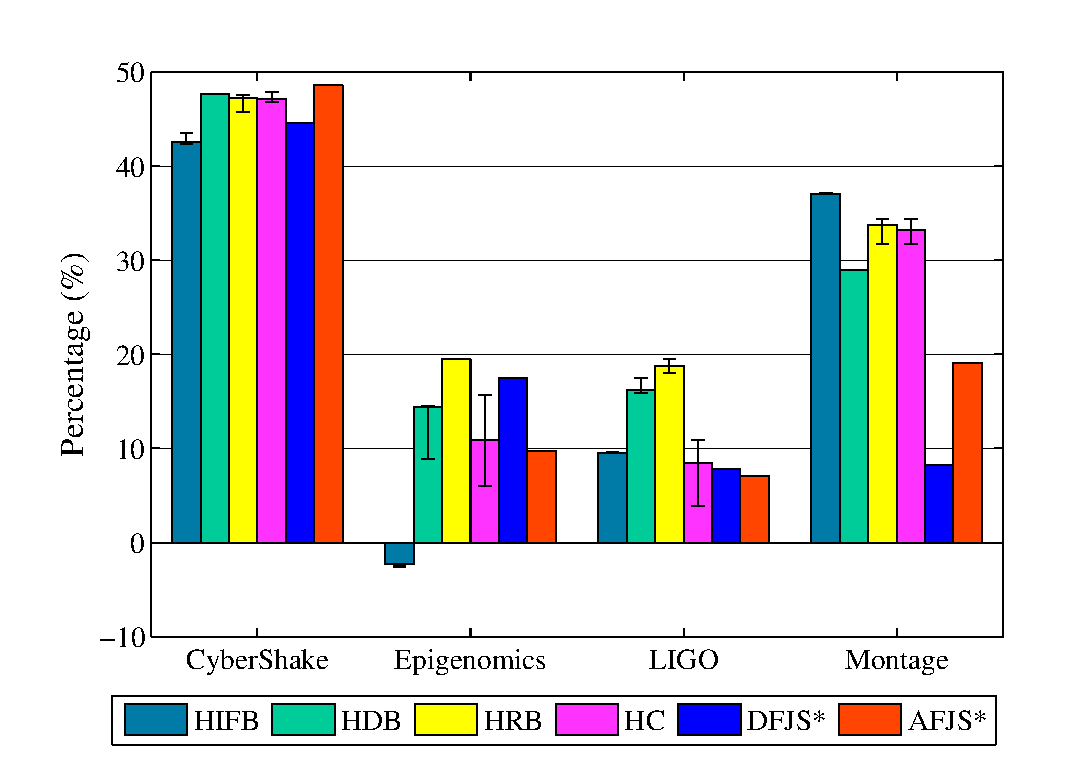
\includegraphics[width=1.0\linewidth]{figures/evaluation/algorithm2.eps}
	\captionof{figure}{Experiment 1: performance gain ($\mu$) over a control execution for six algorithms (*~indicates the tuned performance of DFJS and AFJS).}
	\label{fig:evaluation_algorithm}
\end{figure}

\begin{table}[htb]
	\setlength{\tabcolsep}{12pt}
	\centering
	\small
	\begin{tabular}{c|r|r|r|r}
		& Tasks & HRV &  HIFV & HDV  \\ \hline
		Level & \multicolumn{4}{c}{(a) \textbf{CyberShake}} \\
		\hline
		1 & 4 & 0.309 & 0.03 & 1.22 \\
		2 & 347 & 0.282 & 0.00 & 0.00 \\
		3 & 348 & 0.397 & 0.00 & 26.20 \\
		4 & 1 & 0.000 & 0.00 & 0.00 \\
		\hline
		Level & \multicolumn{4}{c}{(b) \textbf{Epigenomics}} \\
		\hline
		1 & 3 & 0.327 & 0.00 & 0.00  \\
		2 & 39 & 0.393 & 0.00 & 578.00 \\
		3 & 39 & 0.328 & 0.00 & 421.00 \\
		4 & 39 & 0.358 & 0.00 & 264.00 \\
		5 &39 & 0.290 & 0.00 & 107.00 \\
		6 & 3 & 0.247 & 0.00 & 0.00  \\
		7 &1  & 0.000 & 0.00 & 0.00 \\
		8 &1 & 0.000 & 0.00 & 0.00 \\
		9 & 1 & 0.000 & 0.00 & 0.00 \\
		\hline
		Level & \multicolumn{4}{c}{(c) \textbf{LIGO}} \\
		\hline
		1 & 191 & 0.024 & 0.01 & 10097.00 \\
		2 & 191 & 0.279 & 0.01 & 8264.00 \\
		3 & 18 & 0.054 & 0.00 & 174.00 \\
		4 & 191 & 0.066 & 0.01 & 5138.00 \\
		5 & 191 & 0.271 & 0.01 & 3306.00 \\
		6 & 18 &  0.040 & 0.00 & 43.70 \\
		\hline		
		Level & \multicolumn{4}{c}{(d) \textbf{Montage}} \\
		\hline
		1 &49 & 0.022 & 0.01 & 189.17 \\
		2 & 196 & 0.010 & 0.00 & 0.00 \\
		3 & 1 & 0.000 & 0.00 & 0.00 \\
		4 & 1 & 0.000 & 0.00 & 0.00 \\
		5 &49 & 0.017 & 0.00 & 0.00 \\
		6 & 1 & 0.000 & 0.00 & 0.00 \\
		7 &1  & 0.000 & 0.00 & 0.00 \\
		8 &1 & 0.000 & 0.00 & 0.00 \\
		9 & 1 & 0.000 & 0.00 & 0.00 \\
	\end{tabular}
	\caption{Experiment 1: imbalance metrics.}
	\label{tab:evaluation_montage}
\end{table} 



\paragraph{\textbf{Experiment 2}} 
Fig.~\ref{fig:evaluation_datasize} shows the performance gain of HIFB, HDB, HRB and HC for the LIGO Inspiral workflow. The reason we chose the LIGO Inspiral workflow is that it has most significant difference among these methods. It is clear that with the increase of average data size, HIFB performs better and better while HRB performs worse. We don't see much difference of HC and HDB while varying data size. The reason is HIFB is able to capture the structural and runtime information, reducing data transfers between tasks, while HRB focuses on runtime distribution only. Therefore, while the workflow is more data intensive, we observe better performance of HIFB and a worse performance of HRB. HC does not change much since it is randomly merges tasks at the same horizontal level without information about runtime or data dependency. HDB does not change much since its performance gain is already good enough. 


\begin{figure*}[!htb]
	\centering
    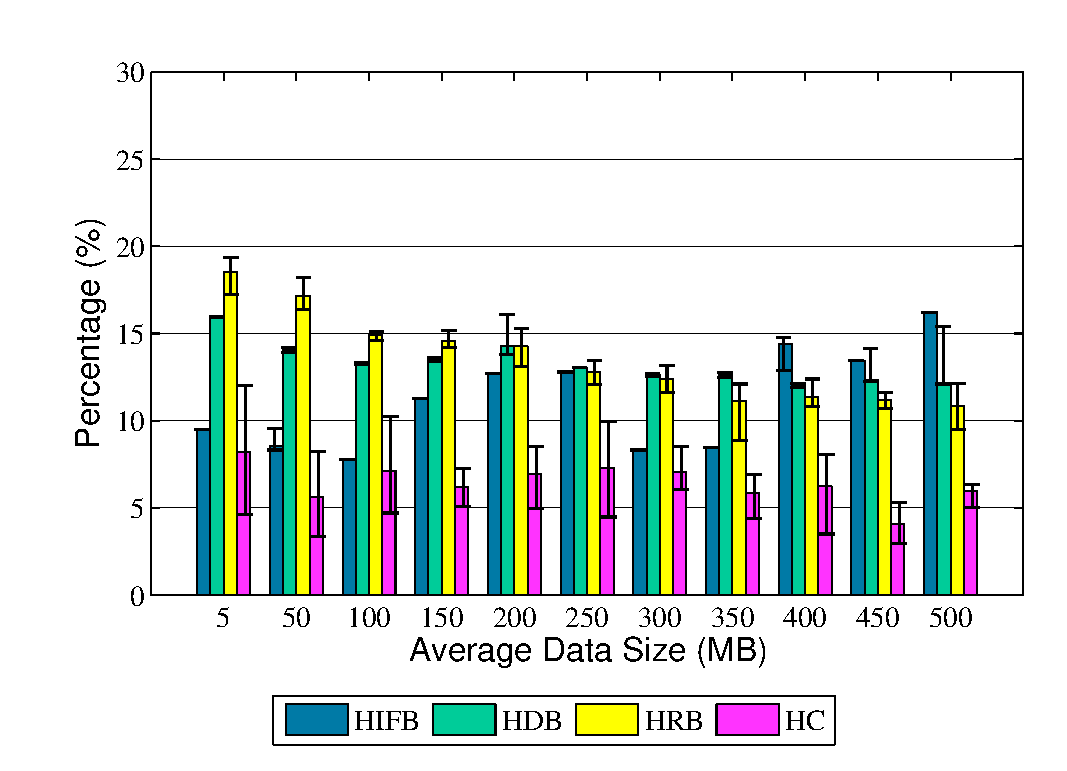
\includegraphics[width=0.7\textwidth]{figures/evaluation/datasize2.eps}
    \caption{Performance Gain over No Clustering with Different Data Size}
    \label{fig:evaluation_datasize}
\end{figure*}

\begin{figure}[!htb]
	\centering
	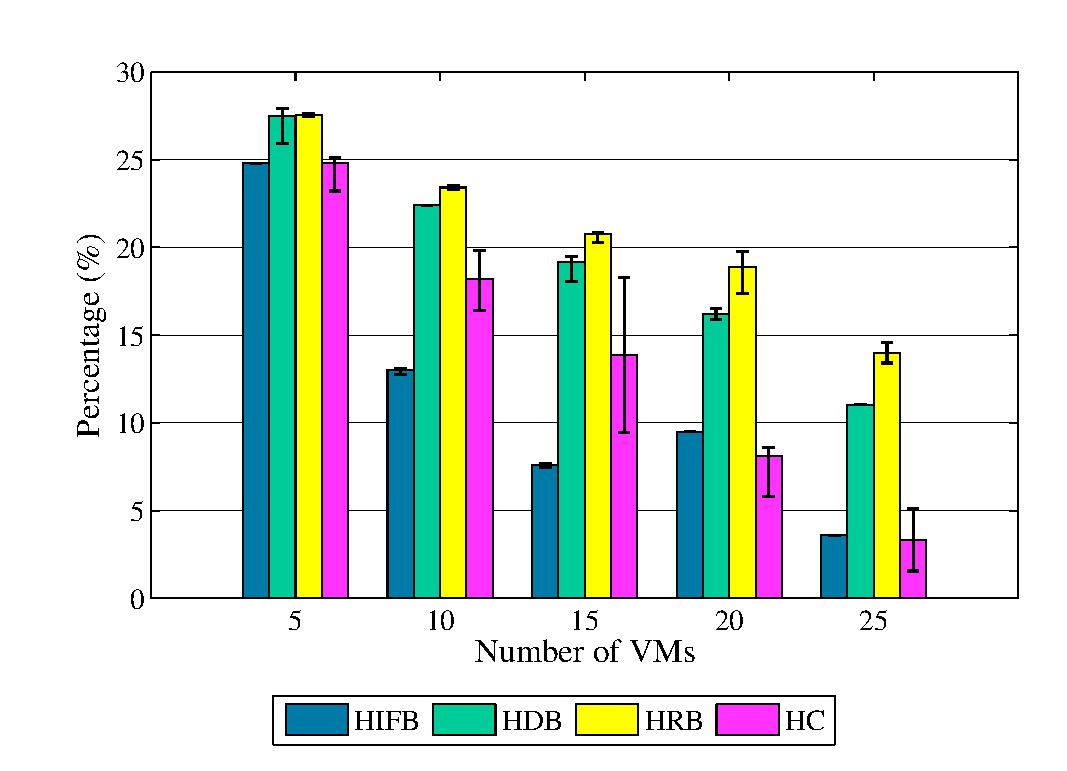
\includegraphics[width=1.0\linewidth]{figures/evaluation/resource1.eps}
	\captionof{figure}{Performance Gain over No Clustering with Different Number of Resources (Average data size is 5MB).}
	\label{fig:evaluation_resource_1}
\end{figure}

\begin{figure}[!htb]
	\centering
	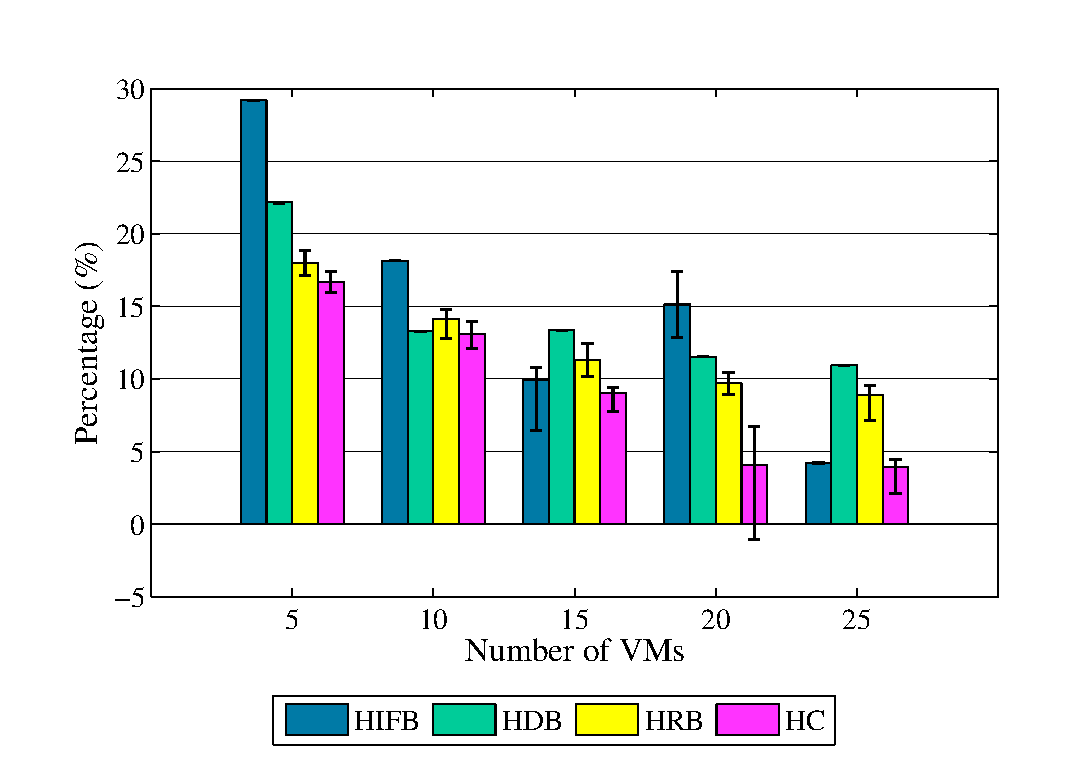
\includegraphics[width=1.0\linewidth]{figures/evaluation/resource2.eps}
	\captionof{figure}{Performance Gain over No Clustering with Different Number of Resources (Average data size is 500MB)).}
	\label{fig:evaluation_resource_2}
\end{figure}




%\begin{figure}[!htb]
%	\centering
%	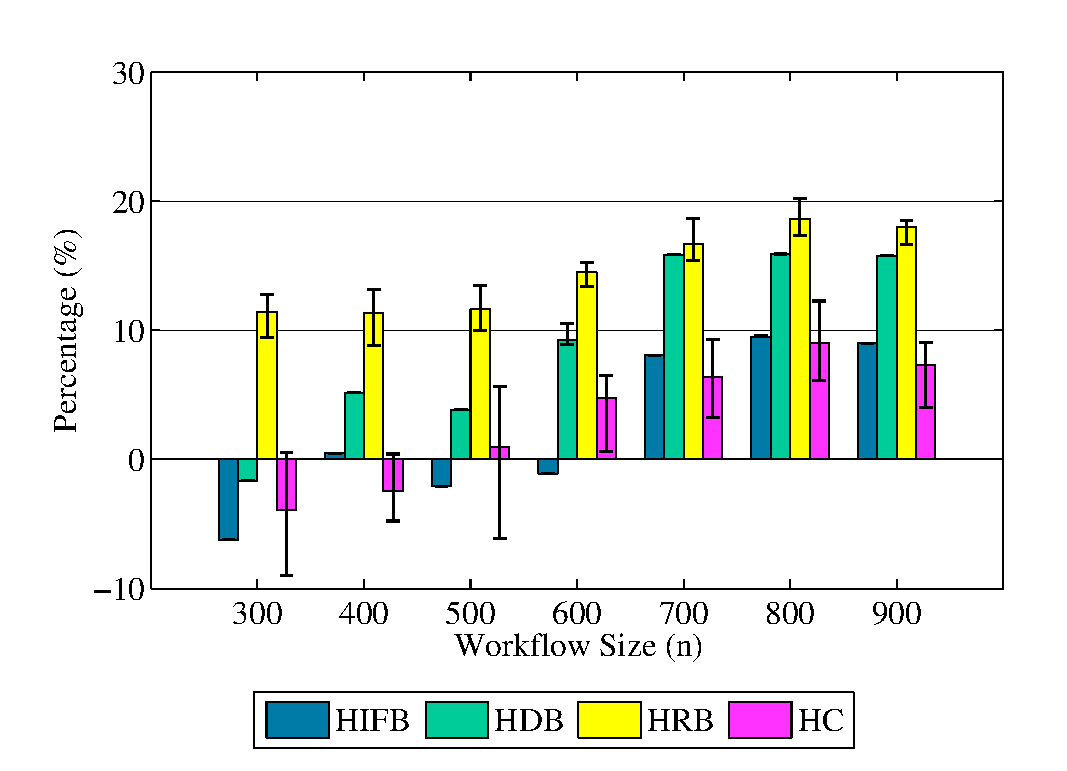
\includegraphics[width=1.0\linewidth]{figures/evaluation/workflowsize.eps}
%	\captionof{figure}{Performance Gain over No Clustering with different Workflow Sizes}
%	\label{fig:evaluation_wfsize}
%\end{figure}

\begin{figure}[!htb]
	\centering
	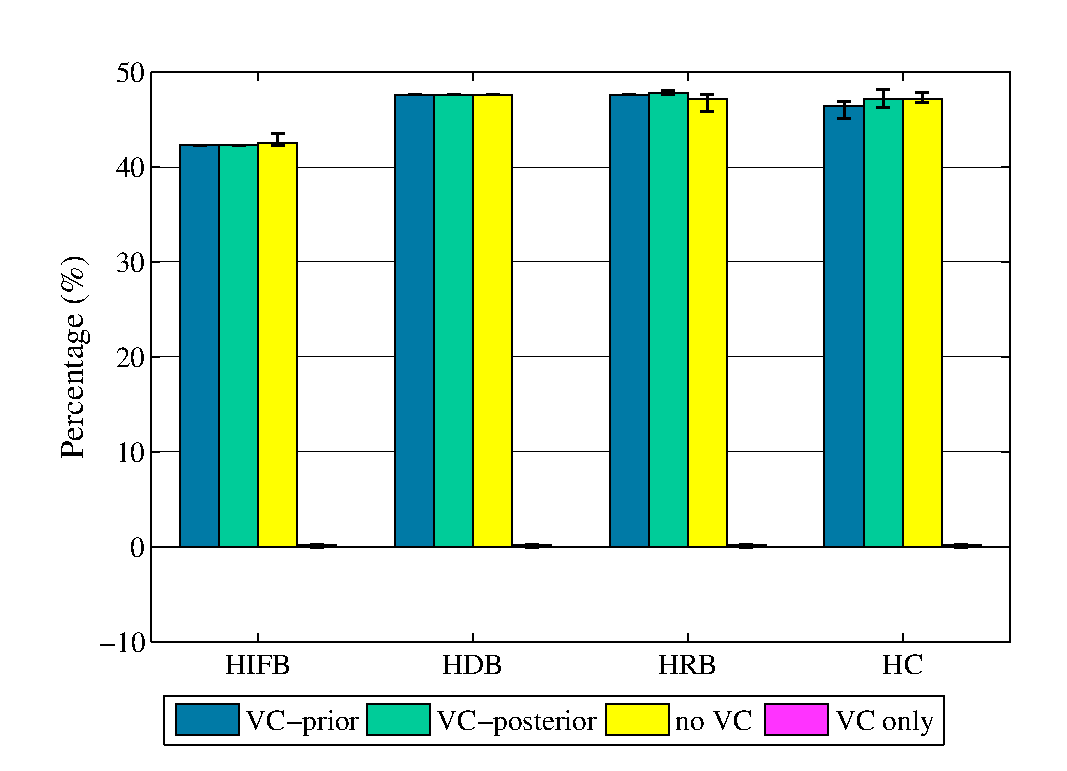
\includegraphics[width=1.0\linewidth]{figures/evaluation/vc_cybershake2.eps}
	\captionof{figure}{Performance Gain over No Clustering for Vertical Methods (CyberShake)}
	\label{fig:evaluation_vc_cybershake}
\end{figure}



\begin{figure}[!htb]
	\centering
    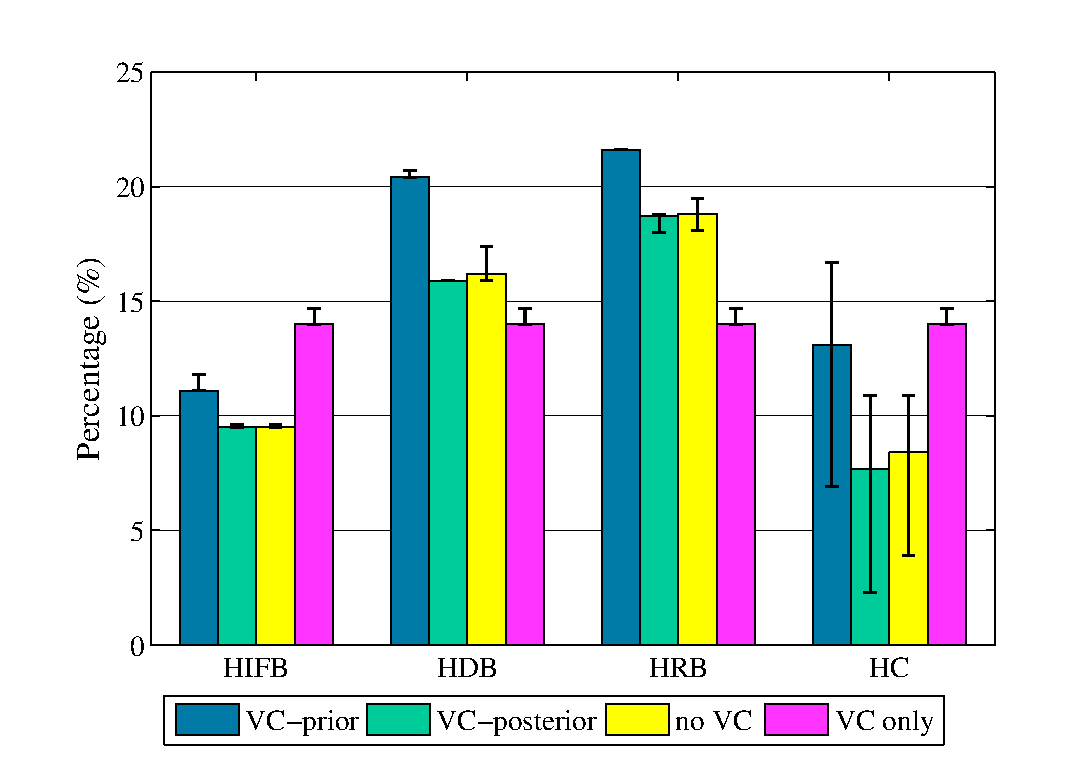
\includegraphics[width=1\linewidth]{figures/evaluation/vc_ligo2.eps}
    \captionof{figure}{Performance Gain over No Clustering for Vertical Methods (LIGO)}
    \label{fig:evaluation_vc_ligo}
\end{figure}


\begin{figure}[!htb]
	\centering
	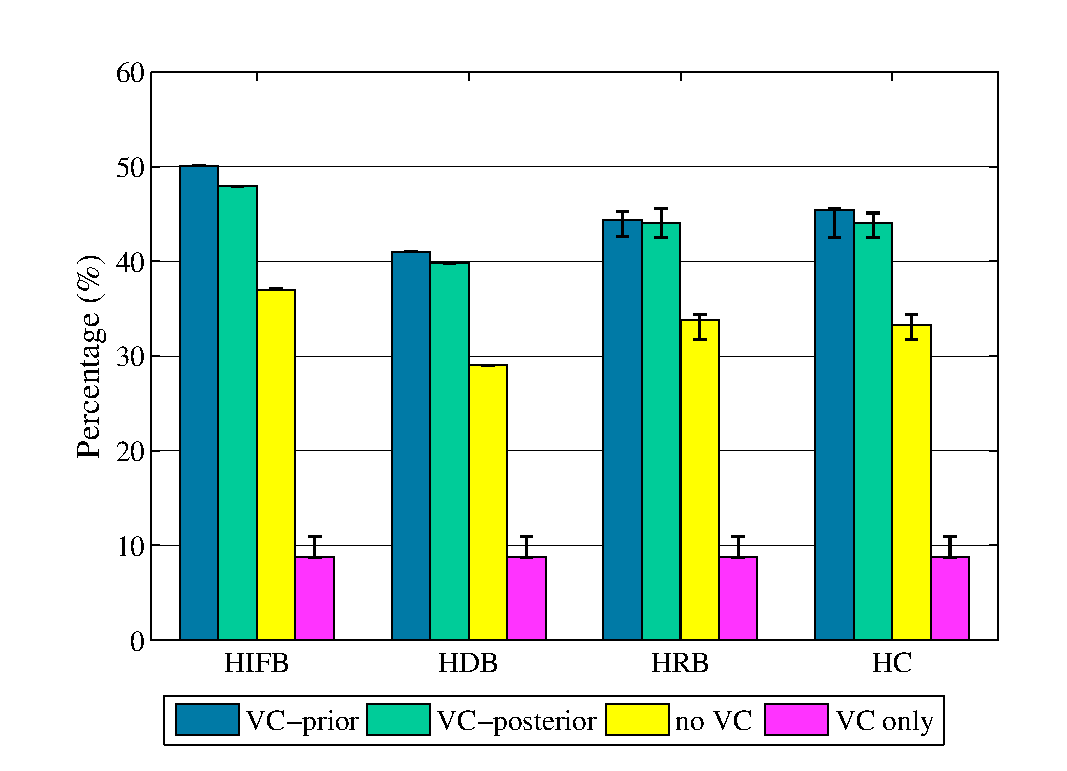
\includegraphics[width=1.0\linewidth]{figures/evaluation/vc_montage2.eps}
	\captionof{figure}{Performance Gain over No Clustering for Vertical Methods (Montage)}
	\label{fig:evaluation_vc_montage}
\end{figure}

\begin{figure}[!htb]
	\centering
	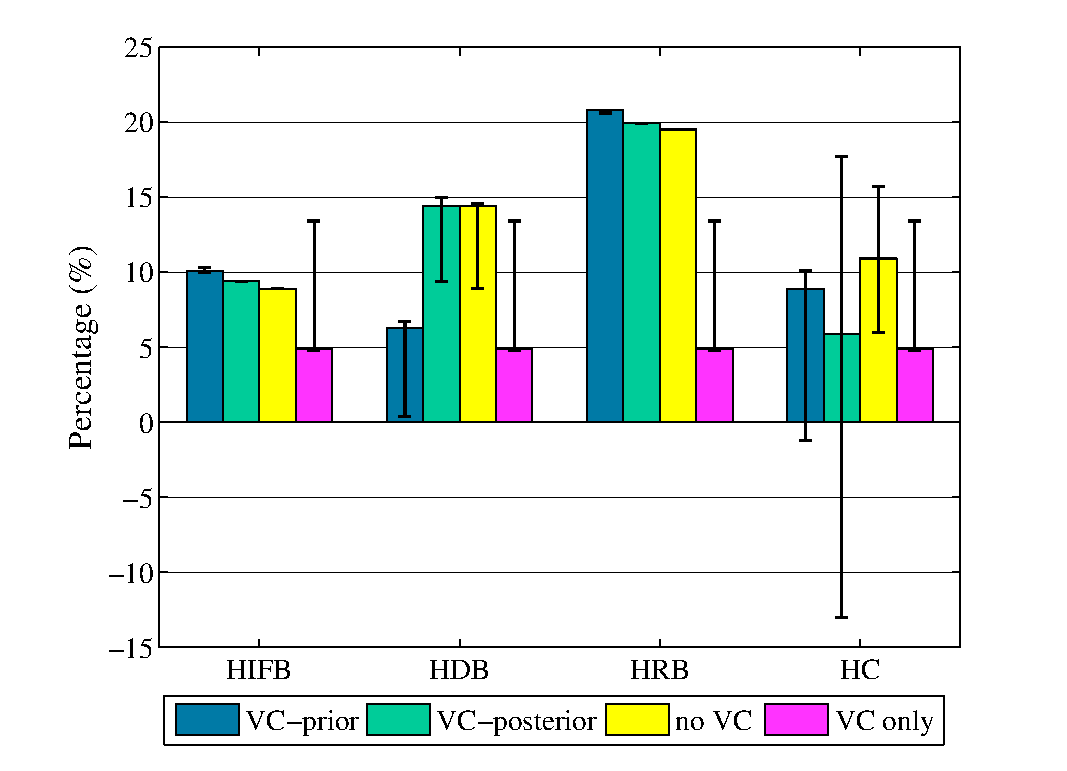
\includegraphics[width=1.0\linewidth]{figures/evaluation/vc_genome2.eps}
	\captionof{figure}{Performance Gain over No Clustering for Vertical Methods (Genome)}
	\label{fig:evaluation_vc_genome}
\end{figure}







\begin{table}[!htb]
\caption{Imbalance Metrics (LIGO after performing VC)}
\label{tab:evaluation_ligo_vc}
\centering
\begin{tabular}{lrrrrrrrr}
\hline
Level & Tasks & HRV   \\

\hline
1,2 & 191 & 0.271  \\
3 & 18 & 0.054 \\
4,5 & 191 & 0.268 \\
6 & 18 &  0.04 \\

\hline
\end{tabular}
\end{table} 


Fig.~\ref{fig:evaluation_resource_1} and Fig.~\ref{fig:evaluation_resource_2} vary the number of VMs with an average data size of 5MB and 500MB respectively. We can see that with the increase of VMs, the performance gain of all of these methods decrease while HIFB and HDB decrease more significantly than HRB and HC. The reason is similar to the case of Fig.~\ref{fig:evaluation_datasize} since HIFB and HDB are data dependency aware. The difference between HDB and HIFB is HDB captures the strong connections between tasks (data dependencies) and HIFB captures the weak connections (similarity in terms of structure). In some cases, HIFV is zero (i.e, Epigenomics) while HDV is less unlikely to be zero. 
%Fig.~\ref{fig:evaluation_wfsize} compares the performance gain of these algorithms by varying the workflow sizes (number of tasks in a workflow). By default, the LIGO Inspiral workflow in our paper has 800 tasks. With the decrease of workflow size, we can see that all of these methods perform worse. The reason is there is less resource contention with the decrease of workflow size and therefore task clustering does not perform well. The performance of HRB is more stable since the increase (or decrease) of workflow size has more significant impact on data transfer (roughly linear increase in runtime and square increase in data transfer). 

Experiment 3: Fig.~\ref{fig:evaluation_vc_cybershake},~\ref{fig:evaluation_vc_ligo},~\ref{fig:evaluation_vc_montage} and ~\ref{fig:evaluation_vc_genome} show the performance gain of combining VC along with our horizontal methods with four workflows respectively. For the CyberShake workflow as shown in Fig.~\ref{fig:evaluation_vc_cybershake}, we do not observe any significant change with VC since CyberShake does not have an explicit pipeline that we can perform vertical clustering (the performance gain of VC only is almost zero). 


For the LIGO Inspiral workflow as shown in Fig.~\ref{fig:evaluation_vc_ligo}, we can see that VC-prior perform better than other combination approaches. The reason is VC-prior increases HRV and allows horizontal methods to improve the performance further while VC-posterior does not have many tasks to merge since horizontal methods change the pipeline structures. Table.~\ref{tab:evaluation_ligo_vc} shows the HRV after we perform VC on the LIGO Inspiral workflow. 

For the Montage workflow as shown in Fig.~\ref{fig:evaluation_vc_montage}, we do see significant improvement with VC (about 15\% more than the case without VC). However, the performance improvement does not distinguish these horizontal methods. The reason is tasks merges by VC (the middle and the tail levels of Montage as shown in Fig.\ref{fig:evaluation_shape_montage})are different from the one merged by horizontal methods (the first two levels in Fig.~\ref{fig:evaluation_shape_montage}). Therefore, the performance of VC-posterior and VC-prior does not differ from each other.  


For the Epigenomics workflow as shown in Fig.~\ref{fig:evaluation_vc_genome}, we observe similar phenomenon in HRB compared to the LIGO Inspiral workflow. As to the performance of HDB, VC-prior merges tasks at the second, third, fourth and fifth level together and thus HDB has less space to further improve the overall runtime. 
 
%HIFB and HDB significantly increase the performance of the workflow execution. Both strategies capture the structural and runtime information, reducing data transfers between tasks, while HRB focuses on runtime distribution, which in this case is none. Fig.~\ref{fig:imbalance_performance} (bottom) shows the performance of the balancing methods for the Epigenomics workflow. When increasing the average data size, only HDB demonstrates significantly improvement related to HC. Investigating the structure of the Epigenomics workflow (Fig.~\ref{fig:imbalance_shape}-bottom), we can see that all tasks at the same horizontal level share the same IFs ($HIFV$ = 0), because each branch (surrounded by dash lines) happen to have the same amount of pipelines. Thus, HIFB has no performance improvement when compared to HC. However, for LIGO (Fig.~\ref{fig:imbalance_shape}-top), $HIFV \neq 0$, thus HIFB improves the workflow runtime performance.  
%The intuition behind this difference between HDB and HIFB is that 
%HDB captures the strong connections between tasks (data dependencies) and HIFB captures the weak connections (similarity in terms of structure). In both workflows, $HDV$ is not zero thus HDB performs better than HC. 






